\documentclass[a4paper,10pt]{article}\usepackage[]{graphicx}\usepackage[]{color}
%% maxwidth is the original width if it is less than linewidth
%% otherwise use linewidth (to make sure the graphics do not exceed the margin)
\makeatletter
\def\maxwidth{ %
  \ifdim\Gin@nat@width>\linewidth
    \linewidth
  \else
    \Gin@nat@width
  \fi
}
\makeatother

\definecolor{fgcolor}{rgb}{0.345, 0.345, 0.345}
\newcommand{\hlnum}[1]{\textcolor[rgb]{0.686,0.059,0.569}{#1}}%
\newcommand{\hlstr}[1]{\textcolor[rgb]{0.192,0.494,0.8}{#1}}%
\newcommand{\hlcom}[1]{\textcolor[rgb]{0.678,0.584,0.686}{\textit{#1}}}%
\newcommand{\hlopt}[1]{\textcolor[rgb]{0,0,0}{#1}}%
\newcommand{\hlstd}[1]{\textcolor[rgb]{0.345,0.345,0.345}{#1}}%
\newcommand{\hlkwa}[1]{\textcolor[rgb]{0.161,0.373,0.58}{\textbf{#1}}}%
\newcommand{\hlkwb}[1]{\textcolor[rgb]{0.69,0.353,0.396}{#1}}%
\newcommand{\hlkwc}[1]{\textcolor[rgb]{0.333,0.667,0.333}{#1}}%
\newcommand{\hlkwd}[1]{\textcolor[rgb]{0.737,0.353,0.396}{\textbf{#1}}}%
\let\hlipl\hlkwb

\usepackage{framed}
\makeatletter
\newenvironment{kframe}{%
 \def\at@end@of@kframe{}%
 \ifinner\ifhmode%
  \def\at@end@of@kframe{\end{minipage}}%
  \begin{minipage}{\columnwidth}%
 \fi\fi%
 \def\FrameCommand##1{\hskip\@totalleftmargin \hskip-\fboxsep
 \colorbox{shadecolor}{##1}\hskip-\fboxsep
     % There is no \\@totalrightmargin, so:
     \hskip-\linewidth \hskip-\@totalleftmargin \hskip\columnwidth}%
 \MakeFramed {\advance\hsize-\width
   \@totalleftmargin\z@ \linewidth\hsize
   \@setminipage}}%
 {\par\unskip\endMakeFramed%
 \at@end@of@kframe}
\makeatother

\definecolor{shadecolor}{rgb}{.97, .97, .97}
\definecolor{messagecolor}{rgb}{0, 0, 0}
\definecolor{warningcolor}{rgb}{1, 0, 1}
\definecolor{errorcolor}{rgb}{1, 0, 0}
\newenvironment{knitrout}{}{} % an empty environment to be redefined in TeX

\usepackage{alltt}
\usepackage{a4wide}
\usepackage{amsmath}
\usepackage{amssymb}
\usepackage[english]{babel}
\usepackage{eurosym}
\usepackage{inputenc}
\usepackage{graphicx}
\usepackage[linesnumbered,ruled]{algorithm2e}
\usepackage{enumerate}
\usepackage{caption}
\usepackage{float}

\title{An analysis on the Metropolis-Hastings algorithm for various iterations}
\author{Kenneth Ruiter (12206909)}
\IfFileExists{upquote.sty}{\usepackage{upquote}}{}
\begin{document}
% setting global settings and loading useful libraries


\maketitle
\newpage

\tableofcontents
\newpage

\section{Introduction}

In statistics, being able to draw from any distribution you like is a very useful tool for analysing your data. Aside from just the 'usual' distributions, some user-defined ones can be hard to sample from directly, when their density is somewhat odd. A well-known way of solving this problem, is by using the Metropolis-Hastings algorithm. This algorithm is a so-called MCMC (Markov Chain Monte Carlo) method to get random samples from such a difficult distribution. In this report we will focus on a particular example of the Metropolis-Hastinds algorithm. We will use the algorithm to estimate the parameters of a simple Ordinary Least Squares regression model, as to easily compare them with the analyitically computed values of the estimates. We will focus on the accuracy of the algorithm by comparing the outputs for a different number of iterations used to compute our estimate.

\subsection{Overview of the report}
In Section~\ref{AD}, we will give more elaborate discription of the Metropolis-Hastings algorithm. We will not explain why it works, however we will go through the algorithm step-by-step. Afterwards, we will randomly generate the data and define some parameters in Section~\ref{Set}. Then the results of the algorithm will be shown and discussed in Section~\ref{Res}. Finally, a short conclusion will be given in Section~\ref{Con}.

\newpage
\section{Algorithm Description}\label{AD}

In this section, the steps involved in the Metropolis-Hastings algorithm will be discussed, using pseudo-code. For this, let $f(x)$ be the density of the distribution that we want to sample from, also known as the target distribution. We will need an initial draw from our sample, so we arbitrarily take $x_0$. We also need an arbitrary second distribution, that we can easily sample from, with density $g(x)$. This distribution will suggest a new candidate for the following draws. We usually take a symmetric distribution, like the Normal distribution, because it makes it easy to compute the acceptance rate of the candidates. This distribution is ususally called the jumping distribution, or sometimes the proposal distribution. The actual steps of the algorithm are shown now.

\begin{algorithm}[H]
    \SetKwInOut{Input}{Input}
    \SetKwInOut{Output}{Output}

    \underline{function run\_metropolis\_MCMC} $(f, g,x_0, iterations)$\;
    \Input{Density function of target distribution $f$, density function of jumping distribution $g$, initial draw $x_0$, number of iterations $iterations$.}
    
    \Output{A vector of the ordered accepted draws, representing draws from the target distribution.}
    \uIf{$intdist$ is exponential}
      {
        Set number of random interarrival times $N$ to $T * intarrpar1$\;
        Randomly generate $N$ interarrival times using an exponential distribution with parameter $intarrpar1$\;
      }
    \uElseIf{$intdist$ is gamma}
      {
        Set number of random interarrival times $N$ to $T * intarrpar2 / intarrpar1$\;
        Randomly generate $N$ interarrival times using a gamma distribution with parameters $intarrpar1$ and $intarrpar2$\;
      }
    \uIf{$cldist$ is uniform}
     {
        Generate $N$ claim sizes using a continuous uniform distribution with parameters $clsizepar1$ and $clsizepar2$\;
     }
    \uElseIf{$cldist$ is exponential}
     {
        Generate $N$ claim sizes using an exponential distribution with parameter $clsizepar1$\;
     }
    \uElseIf{$cldist$ is gamma}
     {
        Generate $N$ claim sizes using a gamma distribution with parameters $clsizepar1$ and $clsizepar2$\;
     }
    Set arrival times to the cumulative sum of the interarrival times\;
    Set levels to the cumulative sum of the claim sizes\;
    Set the premium to $u0 + c * arrivalTimes$\;
    Set the boolean $ruin$ to $min(premium - levels) < 0$\;
    Create a list $ret$ of the arrival times, levels and $ruin$\;
    Return $ret$\;
    \caption{The Metropolis-Hastings algorithm}
\end{algorithm}

\section{Setup}\label{Set}

\section{Results}\label{Res}

\section{Conclusion}\label{Con}

\begin{knitrout}
\definecolor{shadecolor}{rgb}{0.969, 0.969, 0.969}\color{fgcolor}

{\centering 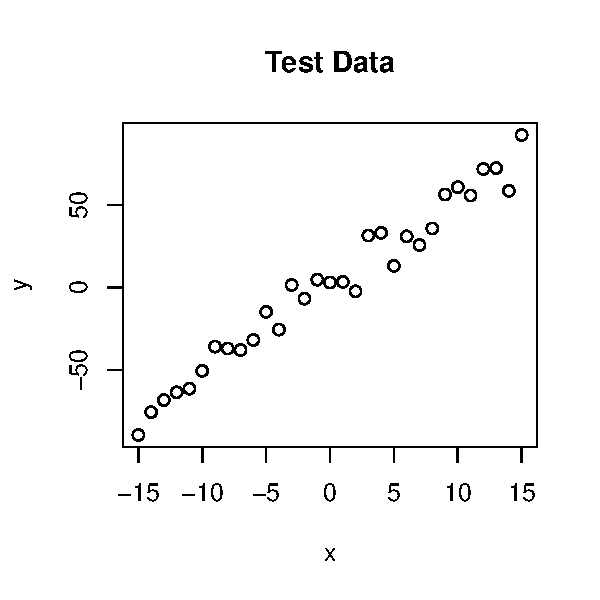
\includegraphics[width=\maxwidth]{figure/setup_functions_and_parameters-1} 

}




{\centering 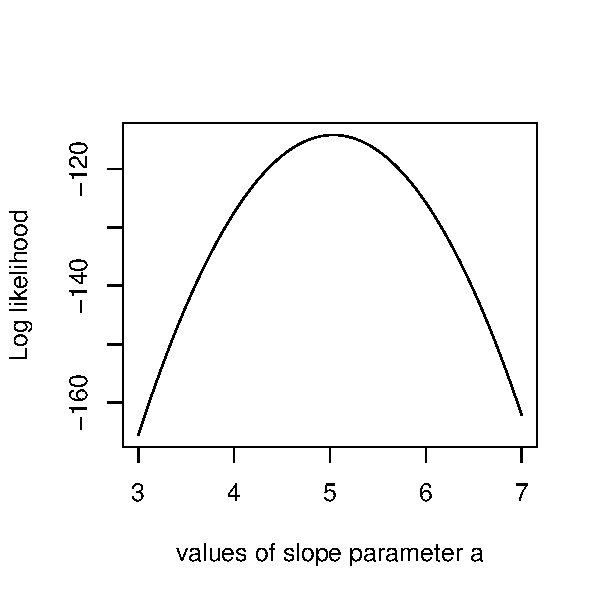
\includegraphics[width=\maxwidth]{figure/setup_functions_and_parameters-2} 

}




{\centering 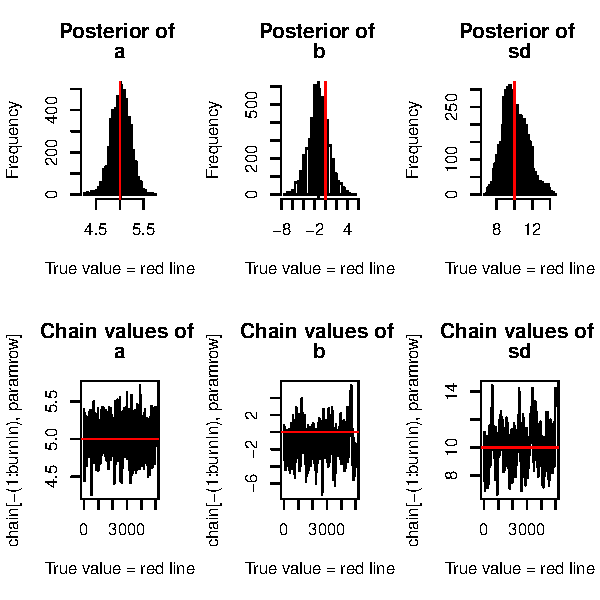
\includegraphics[width=\maxwidth]{figure/setup_functions_and_parameters-3} 

}


\begin{kframe}\begin{verbatim}
## 
## Call:
## lm(formula = y ~ x)
## 
## Residuals:
##     Min      1Q  Median      3Q     Max 
## -28.638  -2.827   0.917   5.319  15.967 
## 
## Coefficients:
##             Estimate Std. Error t value Pr(>|t|)    
## (Intercept)  -1.1176     1.7739   -0.63    0.534    
## x             5.0344     0.1983   25.38   <2e-16 ***
## ---
## Signif. codes:  0 '***' 0.001 '**' 0.01 '*' 0.05 '.' 0.1 ' ' 1
## 
## Residual standard error: 9.877 on 29 degrees of freedom
## Multiple R-squared:  0.9569,	Adjusted R-squared:  0.9554 
## F-statistic: 644.3 on 1 and 29 DF,  p-value: < 2.2e-16
\end{verbatim}
\end{kframe}
\end{knitrout}

\end{document}
